\documentclass[letterpaper,twocolumn,10pt]{article}
\usepackage{usenix-2020-09}

\usepackage{tikz}
\usepackage{pgfplots}
\usepackage{amsmath}
\usepackage{blindtext}
\usepackage{multirow}
\usepackage{graphicx}
\usepackage{caption}
\usepackage{listings}
\usepackage{svg}
\usepackage{hyperref}


%-------------------------------------------------------------------------------
\begin{document}
	%-------------------------------------------------------------------------------
	
	%don't want date printed
	\date{}
	
	\title{CPSC 436A: Final Report}
	
	%for single author (just remove % characters)
	\author{
		{\rm Arpit Kumar}\\
		University of British Columbia
		\and
		{\rm Milo Piccini Noble}\\
		University of British Columbia
		\and
		{\rm Seraj Aldin Abo Sabbah}\\
		University of British Columbia
		\and
		{\rm Zehao Lu}\\
		University of British Columbia
	}
	
	\maketitle
	
\section*{Introduction}
This document outlines the design of our implementation for milestones 1-6. We discuss the reasoning behind our design decisions and detail the issues we encountered. We would like to acknowledge all the help we received from the CPSC 436A team along the way -- thank you! 


\section*{Milestone 1}
%\begin{figure*}[t]
%	\includegraphics[width=\textwidth]{images/dog.jpg}
%	\caption{Woo such a cute dog.}
%	\label{figure:dog}
%	\centering
%\end{figure*}

%We can see a very cute dog in \autoref{figure:dog}. 
%Such a good boy!
%Here is a reference~\cite{jia2023kernel}.

\lstset{
    language=C
}

\begin{quote}
"Simplicity is prerequisite for reliability." \\
\hspace*{\fill} — Edsger W. Dijkstra
\end{quote}

The task for Milestone 1 was to implement the infrastructure for managing physical memory using Barrelfish's capability system. This entailed coming up with our own representation of physical memory and defining all memory operations in terms of this representation. This section explains the design of our representation.

\subsection*{A Model of Physical Memory}
In class, we discussed several approaches to modeling physical memory, including bitmaps, red-black and AVL trees, and a linked list. We decided to use a (singly) linked list representation for one reason and one reason only: simplicity. Given that this was the first milestone, each one of us was relatively unfamiliar with the codebase, thus we wanted to focus on a \textit{correct} solution rather than an \textit{optimal} one. We discuss improvements on our design in a later \autoref{Improvements}.

Each node in the linked list is tied to a single "free" RAM capability (these are passed on to the `init` dispatcher from the CPU Driver). A node can be in one of two states: \textit{free} or \textit{allocated} and stores the size of the free/allocated block. Note that while we do enforce that every node holds unique capability references and that these capabilities point to disjoint address ranges, we do not maintain any particular ordering of the nodes. 


% During the initialization of the memory manager, it is given "free" RAM capabilities. When memory is allocated, these capabilities are retyped into another type, but regardless of type, these new capabilities are "descendants" of the original RAM capabilities. Thus, we capture this parent-child relationship in our mm\_node representations. We have two level of capabilities in each mm\_node. If the node represents a free piece of RAM, the ref will point to the RAM it represents and the parent is set NULL because the ref is already pointing to the "parent" RAMs. If the node represents an allocated RAM/Frame, the ref points to the allocated cap. Now there is a parent RAM, which is the large block of RAM we are allocating from. The offset is based from the "parent" RAM.

\subsection*{Allocating Memory}
To allocate memory, we traverse our linked list to find a memory region that satisfies the allocation requirements, and retype the free RAM capability into another capability of the type specified during the memory manager initialization. Notice that capabilities for allocated memory regions are descendants of the free RAM capabilities. We capture this parent-child relationship in each node by storing a parent capability reference. This reference is set to \verb|NULL_CAP| if the node is free (i.e just points to the free RAM).

Allocation requests may have specific alignment requirements and varying sizes which often result in situations where the allocation starts at an offset from beginning of the free region. Moreover, allocation requests will likely be smaller than the size of the free region. To ensure we don't leak memory, we insert padding nodes to keep track of these fragments. \autoref{figure:mm} illustrates this process.

As to our allocation strategy, we employ the \textit{first-fit} policy. Again, we made this choice since it was simple and the resulting fragmentation isn't too bad for our purposes. We briefly explored a the more efficient \textit{buddy} allocation strategy but we postponed its implementation due to time constraints.

We would also like to point out a subtle bug that we faced when setting up memory allocation. Initially, upon an allocation, we used the same \verb|capref| in our node for that allocation as the one we returned to the calling process. This caused weird errors where our memory manager lost track of large chunks of memory for no apparent reason. The fix was to insert a call to \verb|cap_copy| to ensure the capabilities used internally in our list are not affected by the capability operations performed by the \verb|init| process.

\begin{figure}[h]
	\includegraphics[width=\columnwidth]{report/images/mm-2.png}
	\caption{Keeping track of virtual memory regions}
	\label{figure:mm}
	\centering
\end{figure}

\subsection*{Freeing Memory}
Freeing previously allocated blocks of memory as a whole is essentially the inverse of allocating them and entails coalescing the padding/leftover nodes into a single node. Again, since we do not maintain any particular ordering of the nodes in our list, we are careful to not coalesce discontinuous memory regions.

Our implementation supports partial freeing of previously allocated blocks. To do so, we broke it down to following cases:
\begin{enumerate}
    \item The partially freed address range \textit{has the same start address} as its containing allocated range. In this case, we adjust the offset on the allocated node to align with the end address of the partially freed region. Note that we also call a retype on the allocated nodes's \verb|ref| capability to make sure it is updated to to refer to this new, smaller region of memory. We then create a new capability for the free region and call \verb|mm_add| to keep track of it.
    \item The partially freed address range \textit{has the same end address} as its containing allocated range. This case is identical to the previous one and is handled similarly -- the only difference here is that the "second half" is freed. This is taken into account when retyping capabilities and updating the pointers.
    \item The partially freed address range \textit{does not have the same start or end address} as its containing allocated range. In this case, the allocated region is split into three. The first and third regions are free and are added back into the memory manager by calls to \verb|mm_add| and the second region now refers to the smaller allocated region.
\end{enumerate}

Notice that since we make calls to \verb|mm_add| to keep track of the partially freed regions, once all sub-regions of an allocation are freed, we are unable to coalesce them. This is not ideal - we are essentially introducing "artificial" fragmentation. This may lead to a case where we are unable to satisfy an allocation request despite having enough memory since the representation of a free region is broken up into smaller pieces in our list.


% For the full deallocation, we simply find the node in the linked list and call cap\_destroy to the "ref" in the mm\_node. Then the node is turned into a free node by setting free boolean and reset the caprefs. Furthermore, coaelscing is needed here to avoid external fragmentation. Assuming there are two sibling nodes. We need to check whether they are free and merge them if both of them are free. It is simple because we only need to change the offsets and size of the nodes.\\
% Partial deallocation occurs when only a portion of a memory block is freed. This scenario has three potential cases, described as follows:\\
% \begin{enumerate}
%     \item \textbf{Start Address Matches}:
%         If the start address of the freed region matches the start address of an allocated node, the node is shrunk, and the freed memory is re-added to mm using mm\_add.

%     \item \textbf{End Address Matches}:
%         When the end address matches, the allocated node is shrunk from the end, and the freed region is re-added to mm.

%     \item \textbf{Freeing Middle Part}:
%         When a block is freed in the middle of an allocated node, the original node is divided into two nodes surrounding the freed memory region. The freed memory is then re-added to mm.
% \end{enumerate}

% Because in partial free, we add the free region back to the mm, the order of nodes in the linked list may not match the order in physical memory. Therefore when we are coaelscing the nodes, there are checks to ensure that only those nodes that are neighbours in the physical memory can be coaelsced. \\

\subsection*{Improvements} \label{Improvements}
 Here are a few improvements we can make to improve physical memory management:
 \begin{itemize}
     \item Decouple allocation policy implementation from the implementation of \verb|mm_alloc| in order to experiment with different allocation strategies and determine which one gives the most favorable performance. We aren't quite sure how to judge the fragmentation that results from these policies apart from our theoretical understanding. For a more immediate improvement, we should use the \textit{worst-fit} policy instead of the current \textit{first-fit} since it achieves better fragmentation without any performance penalties.
     \item Memory allocation is a \textit{very, very} frequent operation and a linked list isn't the most performant data structure. We are considering using an AVL tree structure indexed on the base addresses of a region or its size to keep track of the memory regions. This would greatly improve the time it takes to find a viable free memory region ($O(logn)$ versus $O(n)$).
 \end{itemize}




\section*{Milestone 2}
%\begin{figure}[h]
%	\includegraphics[width=\columnwidth]{images/cat.jpg}
%	\caption{A very cute cat.}
%	\label{figure:cat}
%	\centering
%\end{figure}

%See \autoref{figure:cat}, such a cute cat!

\begin{quote}
"Debugging is twice as hard as writing the code in the first place. Therefore, if you write the code as cleverly as possible, you are, by definition, not smart enough to debug it." \\
\hspace*{\fill} — Brian Kernighan 
\end{quote}

The task for Milestone 2 was to implement a system for managing virtual memory. This can be broken down into the following modules


\subsubsection*{A Model of the Page Table}

To map a given physical address to a virtual address on ARMv8, one must install an entry into the corresponding L3 page table. Due to the capability system present in Barrelfish, the user process wishing to perform this mapping must posses a capability to that particular page table. This means that the memory server must keep around an in-memory model of the actual page table. 

There are a number of data structures one could use to encode this information, with the requirements being to maintain fast access and minimal memory footprint. There were two such structures that immediately stuck out:


\begin{itemize}
\item A \textbf{hash-table} would have a minimal memory footprint and provide very fast access. Deciding what to hash on here presents some difficulties, though. A simple approach would be to hash the index bits of the virtual address, and store the L3 page table along with a linked list of its parent page tables at that location. One could always find a necessary L2 page table by simply looking for the 0'th index L3 with those L2 index bits, and so on. This approach is fast! But still involves a number of layers of indirection. If there was a simple way to construct a \textit{flat} hash table to keep track of all of the page table capabilities we needed, that would be an ideal approach.

\item A \textbf{tree }in which each node contains an array of pointers to its children provides both a minimal memory footprint and constant-time lookup. There is a performance hit incurred from introducing between 3 and 6 levels of indirection (depending on whether the array of children is integral or allocated elsewhere), but the structure is simple and easy to manage. On top of the simplicity, the code for this structure models well the mental image of the tree of tables, making reasoning about it far easier. This is the approach we elected to follow through with. See \autoref{figure:page_table}.
\end{itemize}

\begin{figure}[h]
	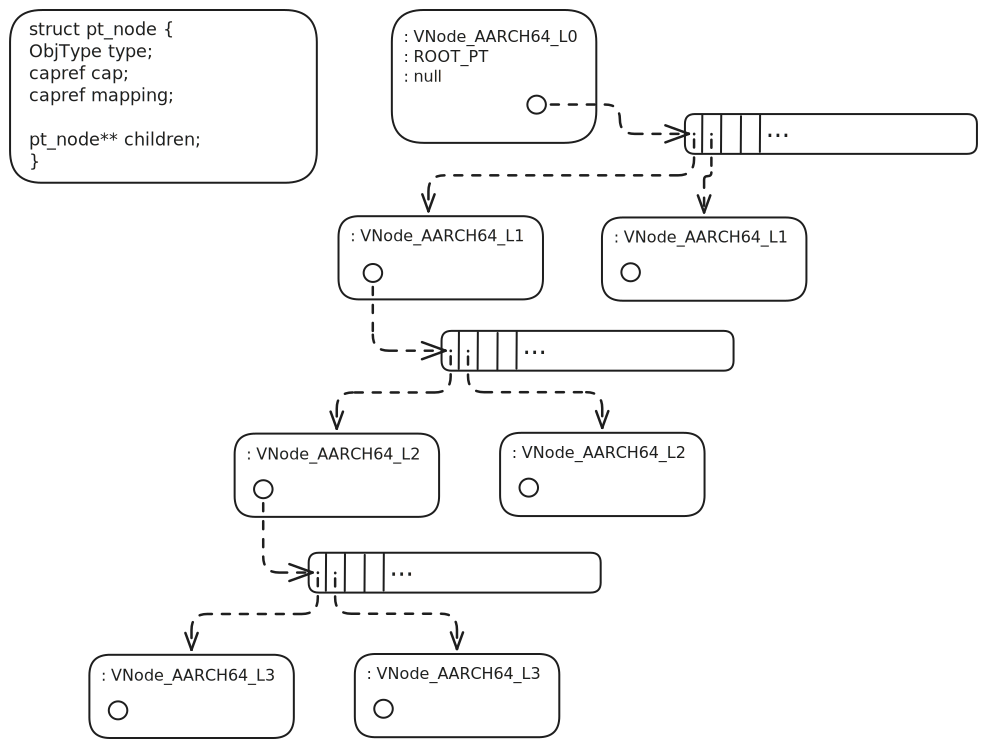
\includegraphics[width=\columnwidth]{report/images/page_table.png}
	\caption{Our representation of the page table}
	\label{figure:page_table}
	\centering
\end{figure}

\subsubsection*{Free, Allocated, and Mapped Memory}

In order to manage and distribute virtual address ranges, we must have some structure to keep track of which regions of the virtual address space are free to be given out, and which are reserved. Additionally, since we require the ability to lazily back these regions with physical memory, we differentiate between allocated (reserved but not backed) and mapped (backed with physical memory). The operations that the virtual memory system must provide are as follows,
\begin{enumerate}
    \item Find a free region of memory and allocate it.
    \item Find a free region of memory and map it
    \item Allocate a specific region of memory
    \item Map a specific region of memory
\end{enumerate}

Some of the operations turn out to be a lot more important than others in Barrelfish. Our key concern in designing this part of our virtual memory system was speed of backing virtual memory in the case of a page fault. Our design makes limited use of allocation and freeing of virtual memory regions, which is explained in the later \autoref{heap} discussing our implementation of the \textbf{heap}. This means that the most frequent virtual memory operation that occurs is a traversal of our virtual memory region structure in order to determine whether an address that triggered a page fault should be mapped (is allocated) or should propagate the page fault as an error (is free).

We prioritize the speed of finding allocated but unmapped regions, and so an AVL tree storing ranges seemed like the obvious approach. By using a comparison function that checked to see if the provided range was a subset of any existing range in the tree, we could keep things balanced nicely. However, due to time constraints and messy development around this milestone, the initial approach we decided on was to keep a linked list of free and allocated regions to fetch from. A mapping operation, then, would remove a node from this list to be stored in an AVL tree. We failed to realize that this is an incredibly expensive operation to be performing for every page fault, and that optimizing the time it took to find a free region would make little difference to the performance of our allocator. See \autoref{figure:vmf_list} for a diagram of our region list.


\begin{figure*}[h] 
	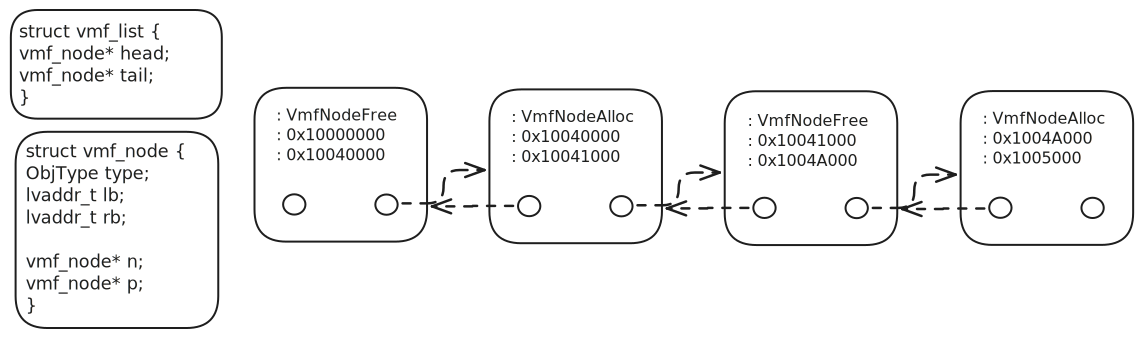
\includegraphics[width=\textwidth]{report/images/vmf_list.png}
	\caption{An initial approach: Keeping track of virtual memory regions}
	\label{figure:vmf_list}
	\centering
\end{figure*}

The page fault handler itself receives upcalls from the barrelfish kernel anytime a given virtual address not backed by any physical memory is touched. The goal of the handler is to verify whether this page fault resulted from a valid memory access, and if so, to perform the mapping operation.

\subsubsection*{The Heap} \label{heap}
Our heap functions by first reserving (allocating) a chunk of the virtual address space larger than the total available memory in the system. We then rely on the page fault handler and our other paging data structures to do the heavy lifting, lazily mapping chunks of this region when accesses occur. Using this approach, our actual \verb|morecore| consisted of very little code, and most of what was written serves setup and teardown.

\subsubsection*{Improvements} \label{improvements}

There are two lines of improvement we wanted to take with our allocation data structures. The first is simple, but halves the level of indirection involved in traversing our in-memory model of the page table. This is simply switching out the \verb|pt_node** children| member of the \verb|pt_node| struct for a \verb|ptr_node* children[]| flexible array member. This allows us to maintain the small memory footprint of L3 page table nodes, which have no children, while simplifying the allocation code. We didn't end up implementing this change due to time constraints.

The second, more involved change to make to our allocation data structures was to rip out our \verb|vmf_list| and simply use AVL trees to keep track of all memory regions. Our thought was that this would remove the $\mathcal{O}(n)$ bottleneck on all of our memory operations and streamline the paging code significantly by unifying our logic for manipulating these regions. However, this did not end up being the case. 


\begin{figure}[h] 
	\includegraphics[width=\columnwidth]{report/images/rpc_lmp(1).png}
	\caption{The free region tree}
	\label{figure:vmf_tree}
	\centering
\end{figure}

In testing, we found that using two separate AVL trees, one for free and allocated regions, the other storing mapped regions, was in fact slower in almost all cases. Allocation suffered a huge performance hit, as now instead of a simple linked list split, we had to rebalance an AVL tree. With the number of nodes we were working with in this memory allocator, this simply did not add up to a reasonable tradeoff.

The unexpected part of this is that mapping and unmapping remained largely unchanged. We can interpret from this that, even with the initial linked list implementation, the cost of AVL tree operations dominates. \autoref{figure:performance} illustrates the performance characteristics of using a linked list vs an AVL tree to implement our free and allocated regions tracking data structure.


\begin{figure}[h] 
	\includegraphics[width=\columnwidth]{report/images/AVL Tree V. Linked List Performance.png}
	\caption{Performance characteristics}
	\label{figure:performance}
	\centering
\end{figure}

\section*{Milestone 3}
\begin{quote}
"Inside every large program, there is a small program trying to get out." \\
\hspace*{\fill} — Tony Hoare
\end{quote}

\lstset{
  language=C,
  basicstyle=\ttfamily\small,
  keywordstyle=\color{blue}\bfseries,
  commentstyle=\color{green!60!black},
  stringstyle=\color{red},
  showstringspaces=false,
  breaklines=true,
  frame=single,
}

Milestone 3 encompasses creating new processes and managing their execution. Key tasks include setting up CSpace and VSpace, loading ELF binaries, configuring the dispatcher, and implementing process management features such as spawn, suspend, resume, and kill.
The implementation covers all core functionalities required for Milestone 3, along with some additional process management tasks. The details are as follows:
%\setcounter{section}{1}
\subsection*{Process Spawning}
\subsubsection*{CSpace Initialization}
\begin{itemize}
    \item A two-level CSpace hierarchy is created for the child process. 
    \item The Level 1 (L1) CNode is initialized using \texttt{cnode\_create\_l1}, and Level 2 (L2) CNodes are set up using \texttt{cnode\_create\_foreign\_l2}.
    \item  Key slots in the CSpace are populated with capabilities such as the dispatcher, root CNode, page tables, and argument frames, following the conventions specified in the Barrelfish documentation.
\end{itemize}

\begin{lstlisting}[caption={CSpace creation with L1 and L2 CNodes}, label=lst:cspace_creation]
errval_t setup_cspace(struct spawninfo *si) {
    // Create the L1 CNode
    errval_t err = cnode_create_l1(&si->l1_cnode_cap, &si->l1_cnode_ref);
    if (err_is_fail(err)) return err;

    // Create L2 CNodes and link them in the L1 CNode
    for (size_t i = 0; i < ROOTCN_SLOTS_USER; ++i) {
        err = cnode_create_foreign_l2(si->l1_cnode_cap, i, &si->l2_cnodes[i]);
        if (err_is_fail(err)) return err;
    }
    return SYS_ERR_OK;
}
\end{lstlisting}


\subsubsection*{VSpace Initialization}
\begin{itemize}
    \item A virtual address space (VSpace) is set up for the child process.
    \item The L0 page table is created using \texttt{vnode\_create}, and mappings for ELF sections are established using \texttt{paging\_map\_fixed\_attr}.
    \item A default slot allocator is initialized to support subsequent memory allocation for the child.
\end{itemize}

\begin{lstlisting}[caption={Setting up the VSpace for the child process}, label=lst:vspace_setup, language=C]
errval_t setup_vspace(struct spawninfo *si) {
    // Initialize the slot allocator
    // ... removed code
    
    // Step 1: Allocate a slot for the L0 page table
    //... removed code

    // Step 2: Create the L0 page table for AARCH64
    err = vnode_create(si->vspace, ObjType_VNode_AARCH64_l0);
    if (err_is_fail(err)) {
        // ... handle errors
    }

    // Step 3: Initialize paging state with the L0 page table
    err = paging_init_state_foreign(&si->process_paging_state, 0, si->vspace, &si->default_sa.a);
    if (err_is_fail(err)) {
        // ... handle errors
    }

    //... removed code that sets up RAM Capability

    return SYS_ERR_OK;
}
\end{lstlisting}

\subsection*{ELF Binary Loading}
Loading the ELF binary into the child's virtual address space (VSpace) is a critical step in process spawning. The goal is to map program segments to specific virtual addresses as specified in the ELF file's program headers. This involves parsing the ELF file, allocating frames for the segments, and performing the necessary mappings. The steps include:

\begin{itemize}
    \item \textbf{Parsing the Program Headers:} Each program segment is described in the ELF file's program headers. These headers specify the virtual addresses and sizes of the segments to be loaded into the process's VSpace.
    \item \textbf{Allocating Frames:} For each segment, a frame is allocated to hold its data. The size of the frame is determined by rounding up the segment's size to the nearest page boundary.
    \item \textbf{Mapping Frames to VSpace:} The allocated frame is mapped into the child's VSpace at the specified virtual address.
\end{itemize}

\subsubsection*{Challenges and Solutions}
\paragraph{Handling VADDR\_OFFSET Issues:} During implementation, we encountered an issue where the virtual address specified in the ELF file was smaller than \texttt{VADDR\_OFFSET}, which was previously assumed to be the smallest virtual address allowed for allocation. This assumption stemmed from the notion that the 1GB offset was reserved for booting. However, further investigation revealed that this reservation only applies to the \texttt{init} process, and the child process is free to allocate memory in the 0–1GB region. To accommodate this, we removed the relevant assertions from M2.

\paragraph{Unaligned Virtual Addresses:} Another challenge was that the specified virtual address for some segments was not aligned to the page size (4KB). This violated the earlier M1 assertion that all allocated physical memory should be aligned to 4KB boundaries. To address this:
\begin{itemize}
    \item The base address was adjusted using \texttt{ROUND\_DOWN} to align it with the page size.
    \item The frame size was increased to include the unaligned portion by adding the offset difference.
    \item During mapping, the frame was mapped starting at the specified base address, leaving the initial unaligned portion unused.
\end{itemize}
This approach minimizes waste, as at most only 4KB of memory is unused.

\begin{lstlisting}[caption={Mapping ELF segments with alignment considerations}, label=lst:elf_mapping, language=C]
static errval_t elf_allocate(void *state, genvaddr_t base, size_t size, uint32_t flags, void **ret) {
    struct spawninfo *si = (struct spawninfo *)state;

    // Align base and size to page boundaries
    genvaddr_t aligned_base = ROUND_DOWN(base, BASE_PAGE_SIZE);
    size_t aligned_size = ROUND_UP(size + (base - aligned_base), BASE_PAGE_SIZE);

    // Allocate and map the memory
    // ... removed code

    // Map into the parent's VSpace
    // ... removed code

    // Map into the child's VSpace
    // ... removed code
    
    *ret = local_addr + (base - aligned_base);
    return SYS_ERR_OK;
}
\end{lstlisting}

\paragraph{Global Offset Table (GOT):} Once the ELF segments are mapped, the Global Offset Table (GOT) is located using ELF section headers. The GOT base address is then used to initialize the dispatcher registers, enabling runtime resolution of global variables and facilitating shared library support.

By addressing these challenges, we ensured that the ELF loader correctly handles real-world binaries, even with complex memory layout requirements.

\subsubsection*{Dispatcher Setup}
\begin{itemize}
    \item A dispatcher control block (DCB) is allocated and mapped into both the parent’s and child’s address spaces. 
    \item The dispatcher is initialized in disabled mode, with fields such as core ID, domain ID, and the program counter set appropriately.
    \item The \texttt{armv8\_set\_registers} function initializes the GOT base and entry point for the dispatcher.
\end{itemize}

\begin{lstlisting}[caption={Initializing the dispatcher fields}, label=lst:dispatcher_init, language=C]
// Access the dispatcher structure fields
struct dispatcher_shared_generic *disp = get_dispatcher_shared_generic(handle);
struct dispatcher_generic *disp_gen = get_dispatcher_generic(handle);

// Initialize dispatcher fields
disp->disabled = 1;                         // Start in disabled mode
disp_init_disabled(handle);                 // Initialize disabled state
disp_gen->core_id = disp_get_core_id();     // Set the core ID for the child
disp_gen->domain_id = domain_id;            // Assign the domain ID
si->pid = domain_id;                        // Store the domain ID in the spawninfo struct
\end{lstlisting}


\subsubsection*{Argument Passing}
\begin{itemize}
    \item  Command-line arguments are parsed and stored in a dedicated arguments frame in the child’s address space.
    \item  The \texttt{spawn\_domain\_params} structure is populated with pointers to the arguments in the child’s VSpace, ensuring proper alignment and null-termination.
\end{itemize}

\subsection*{Process Management}
\subsubsection*{Start, Suspend, Resume, and Kill}
\begin{itemize}
    \item Processes are started by invoking their dispatcher capability, transitioning them to the \texttt{RUNNING} state. Every new process gets assigned a PID by the process manager.
    \item Suspend and resume functionality is implemented by manipulating the dispatcher’s state in the run queue.
    \item Processes can be terminated (killed) by removing their dispatcher from the run queue and setting their state to \texttt{KILLED}.
\end{itemize}


\subsubsection*{Tracking and Cleanup}
\begin{itemize}
    \item A linked-list data structure is used to keep track of processes, storing information such as name, PID, and capabilities.
    \item Although full cleanup of resources is not yet implemented, the framework is in place to traverse and reclaim allocated resources.
\end{itemize}

\subsection*{Optimization and Improvements}
\begin{itemize}
    \item Implement full cleanup of process resources and automatic updates to the process tracking structure upon termination.
    \item Improve the PID assignment as it may overwrite the running PIDs if the number gets too large
\end{itemize}

\section*{Milestone 4}

\begin{quote}
"The single biggest problem in communication is the illusion that it has taken place" \\
\hspace*{\fill} — George Bernard Shaw 
\end{quote}

Now that we have more than a single protection domain, we need a way to communicate between them. In a traditional operating system, one can imagine wanting to be able to request that another process be killed so that a task manager might work, for example. This inter-process communication is even more fundamental to the operation of Barrelfish due to the lack of services in the kernel. When we spawn a new process, if that process wants RAM, it must ask for it from some other process that has capabilities to RAM already. In some sense, IPC is the glue that holds Barrelfish together. 

\subsubsection*{What We're Working With} \label{wwww}
Barrelfish comes with a library for transferring data and capabilities between dispatchers (that this is between dispatchers is important) already, in the form of Lightweight Message Passing. This library allows for non-blocking IPC by invoking a (retyped) capability to the other processes dispatcher, which pulls the kernel into the fray to work a little magic. On top of these raw endpoint capabilities, we have provided for us a channel abstraction, giving rise to "LMP Bindings" and the ability for a thread to wait for a message on such a channel.

Our goal with this milestone was to implement a fast and reliable framework for Remote Procedure Calls between protection domains, built on top of the LMP Channel abstraction. RPC aligns well with the kind of functionality we want out of this system: If a process wants more memory, we're fine with a synchronous call to request it. We also only need very small messages, since we can provide stubs for each of the functions. This means any single call can be made quite quickly. Given we'll be implementing printing to the terminal via this mechanism, our design has to minimize latency.

These operations are core to the function of Barrelfish, so we wanted them to be painless to use, easy to extend, fast, and most of all to seamlessly integrate with UMP (M6) when messages are passed across cores. We succeeded in some of these things.

\subsubsection*{A Messaging Layer Protocol} \label{msg_protocol}

To define a protocol, we need a conception of what a message looks like. The underlying LMP endpoints support transferring up to 8 words at a time, and channels give us a way of blocking and waiting on the dispatch/receipt of these packets. To enforce structure on two ends of a connection, one needs data that describes structure. If there's just one type of message, this can simply be globally agreed upon and fixed.  Given the number of possible RPC subroutines, we need some extra information to be sent with the message itself. We decided to sacrifice 1 word of payload space to pack in information about the length of the payload, its type (i.e. what sort of call we are making -- this lets us agree upon structure on each end), and some other information that is needed for handling messages larger than a single payload. With a message format in place, the task of both the client and server becomes marshalling and unmarshalling messages, and making their respective local function calls -- we have (semi) successfully decoupled our RPC from the underlying transport protocol.

\begin{lstlisting}[caption={RPC Structs}, label=lst:rpc_structs, language=C]
union rpc_hdr {
    struct {
        uint32_t pld_len;
        uint8_t type
        ...
    };
    uint64_t hdr_val;
};

struct rpc_msg {
    struct capref cap;
    union rpc_hdr hdr;
    uintptr_t pld[];
};
\end{lstlisting}

\subsubsection*{The Handshake} \label{handshake}

With an idea of \textit{what} we want to send in mind, we have to actually establish a connection. To keep the latency of each message low, Barrelfish borrows the concept of an explicit 'binding' from LRPC. That is, an LMP channel is persistent over the whole lifetime of a spawned process. Producing this binding is not a particularly interesting design choice, as there's a relatively fixed order. However, as a consequence of our choice to use \hyperref[sec:extending]{shared memory} to handle large messages, we introduce a small amount of complexity. Since all OS services live in the \verb|init| process (again, this is a design decision we made in light of time constraints), any spawned process must first share its endpoint capability to \verb|init| which in turn returns the capability to the shared memory buffer used to handle arbitrary sized messages. This exchange of capabilities is what constitutes our LMP handshake.

\begin{figure}[h!] 
	\includegraphics[width=\columnwidth]{report/images/handshake.png}
	\caption{The LMP Handshake}
	\label{figure:handshake}
	\centering
\end{figure}

\subsubsection*{The Big Picture} \label{sec:big_picture}

The final design of our message passing system can be seen in \autoref{figure:big_picture}. The \verb|burb| library sits at the core of this, handling marshalling/unmarshalling, dispatch logic and receiving messages. \verb|burb| is given an RPC message struct and returns an RPC message struct, hiding all of the underlying LMP logic away. Recall that our architecture stuffs all of the functionality of a memory server, terminal server, and process server into \verb|init|. On the server side then, \verb|burb| takes the form of a generic receive handler that is always registered, forwarding payloads to server-specific functions.

One key observation we made was that a given LMP channel is dispatcher to dispatcher, and hence the introduction of multiple threads on each process meant working with care. The simplest approach in this case was to enforce an invariant and make RPC send/receive pairs atomic. We have a mutex associated with each binding, and the thread making a call acquires the lock before sending a message, releasing it only after it has received a response. 

\subsubsection*{Flaws} \label{sec:flaws}

There are a number of flaws in this approach. The first and most obvious thing is that it severely limits the kinds of RPC calls we can make. Our invariant is that a call is always initiated by a client, and that this call may be treated as a single operation. This assumption was quickly violated when we considered implementing \verb|proc_mgmt_register_wait|, an RPC call that tells a thread to suspend until a specified process is killed. This call is \emph{open}, and with our current design, this could potentially intercept all other calls to the process hosting the suspended thread. We ended up not solving this issue. Perhaps more troubling was our assumption that the server would never want to send a message to a client without the client asking first. This immediately ruled out client-to-client communication via the server process and made a large chunk of M6 totally unviable.

It's worth noting that LMP channels are reliable, so we don't worry about messages failing to send. However, we have no time-out mechanism. If for whatever reason a thread is not able receive a message it expects, not only will it hang, but no further RPC calls will be able to be made by any thread on that process.

Lastly, as mentioned earlier, we decided to house all OS services in the \verb|init| process. This is less than ideal because this limits concurrent access to distinct services. It also means that if the \verb|init| process stops running, access to all services is lost. An ideal approach would have a process for each service along with a name server to enable service discovery.


\subsubsection*{Handling Large Messages} \label{sec:extending}

So what if we want to send messages larger than 7 words? There are a number of potential approaches. One choice is to simply split the message into many LMP messages, associate with each on a sequence number, and reconstruct the message on the other side of the channel. This is slow because we have to context switch for each message, and introduces plenty of opportunities for mistakes to be made in reconstructing the message. Another, arguably simpler approach, is to just share some memory between each process. In our design, we keep these messages synchronous and use LMP to transfer a header describing the message we've written to the shared memory frame. We support arbitrarily sized messages, but with an entire page of memory to work with, the vast majority of messages will only require a single read from this buffer. To illustrate the difference in performance, we have provided benchmarks in \autoref{figure:performance_lmp}, comparing shared memory to multiple LMP messages. This is cropped for readability. 
\begin{figure}[h!] 
	\includegraphics[width=\columnwidth]{report/images/Message Passing via LMP v. Shared Memory.png}
	\caption{Performance characteristics}
	\label{figure:performance_lmp}
	\centering
\end{figure}

And now without cropping (clearly, the number of context switches in the approach using raw LMP payloads dominate the time it takes to share 1 page worth of data and is multiple order of magnitudes slower than using a shared memory buffer).
\begin{figure}[h] 
	\includegraphics[width=\columnwidth]{report/images/Message Passing via LMP v. Shared Memory(1).png}
	\caption{Performance characteristics}
	\label{figure:performance_lmp_uncrop}
	\centering
\end{figure}

\begin{figure*}[h] 
	\includegraphics[width=\textwidth]{report/images/rpc_lmp.png}
	\caption{Our RPC System Design}
	\label{figure:big_picture}
	\centering
\end{figure*}


\section*{Milestone 5}
\begin{quote}
"The free lunch is over. Now welcome to the hardware jungle." \\
\hspace*{\fill} — Herb Sutter 
\end{quote}

The main focus of M5 was to bring up another core. This is where we start to get a sense for Barrelfish as a multikernel operating system. Barrelfish operates under the assumption that no operating  system state is shared between cores. Each core runs its own CPU driver, each of which is like its own microkernel. This is a key part of why Barrelfish supports running on heterogenous hardware, as each CPU driver may be built for a different architecture. On each core, a privileged user-space process called the Monitor (in our case \verb|init|) serves both to handle long-running operations that the kernel itself might not be able to handle (due to its stateless, non interruptable nature, we don't want to simply hang while a capability is deleted) and to communicate with monitor processes on other cores. With this architecture in mind, we also need a way of providing basic communication between cores. We will, in fact, use a shared memory frame (as in our implementation of M4, and as we will expand on in M6).

\subsubsection*{The Process} \label{sec:m5_process}

Much like M3, the approach here is fairly formulaic. There are a set number of steps one must take to boot a new CPU driver on a second core. 

\begin{enumerate}
    \item Allocate memory: We need to provide RAM for the kernel .bss segment, RAM for the init process on the new core, RAM for our communication channels, and RAM to retype into a Kernel Control Block (KCB).
    \item Create KCB \& Coredata data structures: The KCB is the object holding references to all of a running kernel’s state, while Coredata provides the boot parameters to the new CPU driver.
    \item Load the Boot driver and CPU driver: Since there is no shared OS state, we need to load a whole new copy of the CPU driver into RAM. Further, the CPU driver assumes that there is a default kernel page table available upon boot, and that the MMU is enabled. This is handled by the boot driver, which does the last required bootstrapping required to jump into the CPU Driver.
    \item Clean the cache: Since the boot driver starts with the MMU uninitialized, it's important to make sure that everything it needs access to is actually in RAM, not hidden away in some dirty cache line of our current core.
    \item Call spawn: Here we invoke the kernel capability, which abstracts away all of the hardware magic, performing some boot protocol based on platform to start the boot driver. This then spins up the CPU Driver, and we have a new core running.
\end{enumerate}

\subsubsection*{Communication} \label{sec:m5_communication}
The communication channel between cores is a region of shared memory for which the details are passed via the CSpace when booting the new core. In this milestone, this channel was unidirectonal, meaning processes running on the BSP core may make requests to processes on other cores, but not the other way around. We realized in M6 that a simple way to implement bidirectional communication was just two have two producer-consumer structures, "facing" opposite directions occupying the same shared frame. The upper half could be dedicated to reading on core0, writing on core1, and vice versa.

To actually use this channel, and in the absence of any mechanism similar to waitsets, we decided it would be best to have the reader continuously poll the shared memory. Here we had two choices, either
\begin{enumerate}
    \item Bring up a thread in each init process, or
    \item Spawn a new process on each core to serve as a UMP server
\end{enumerate}

\subsubsection*{Complications} \label{sec:m5_complication}

Our initial approach was to work with a polling thread, since that fit our current design more cleanly (given that every server so far had lived inside init), but we ran into many issues with threading. As it turns out, we did \emph{not} have working threads as we had assumed, and made a few fundamental mistakes in understanding. One of these was the misinterpretation of \verb|_onthread| functions, not realizing that these were named as such not because they ran on each new thread, but that they were designed to run in a separate thread on the process they were invoked on. Our thread stack had also been allocated half the size it needed. We fixed these only upon tackling M6.

Since at this point threads were not working, we decided on the approach of spawning a new process. This meant that all messages over the channel had to be forwarded via LMP to init to actually be executed, giving up any performance gains that shared memory might have offered. This also led to poking a lot of holes in our M4 API, further complicating M6 work.

\subsubsection*{Taking "Turns"} \label{sec:m5_turns}

Once we had a polling thread, we needed some sort of mechanism to make sure we weren't reading partially written data. For this, we borrowed an idea from Sequence Locks, and implemented a "turn" based synchronization system. This was a simple way of ensuring that a single-producer single-consumer queue is read on the correct order. We would learn in M6 that in fact memory barriers are key to synchronization across cores on ARM due to its weak memory consistency model. The turn is just a single bit in our buffer data structure that signals whether it is time to read or write. This "turn" based mechanism is demonstrated in \autoref{figure:spawn-call-graph}.

\begin{figure}[h!] 
	\includegraphics[width=\columnwidth]{report/images/m5-graph.png}
	\caption{Call graph outlining the steps that take place when a request to spawn a process is made across cores}
	\label{figure:spawn-call-graph}
	\centering
\end{figure}

\subsubsection*{Further Challenges} \label{sec:m5_chals}
Since we had no waitsets to rely on, our implementation diverged quite heavily from the event driven nature of our previous code. The ability to register a callback made reasoning about LMP communication quite simple, but in our M5 implementation we had to manually handle each message at time of receipt. This didn't fit well with the RPC interface and caused more holes to be punched.

Similarly, to get our unidirectional channel to function we had made many assumptions about communication. These compounded on those we'd made in M4, coming back to bite us in the implementation of M6. 


\section*{Milestone 6}
\begin{quote}
"I have not failed. I've just found 10,000 ways that won't work." \\
\hspace*{\fill} — Thomas A. Edison
\end{quote}

Ah, the last milestone. Now that we have the ability to spawn an additional core, the goal of this milestone was to implement a full inter-core messaging and RPC system by extending our work from M4. We were fairly confident in our conceptual understanding of URPC, but faced several technical and non-technical challenges and we eventually ran out of time before we could implement a working solution. We try to describe our idea, what worked, and what didn't work in this final chapter.

\subsubsection*{The Idea} \label{sec:the_idea}
The idea behind this milestone was to take advantage of shared memory and cache coherency to implement a really fast messaging system between cores. While sharing memory is great when it comes to performance, we had to be extra careful in how we were handling reading/writing to shared memory given Barrelfish's weak memory consistency model. In particular, this meant our ring-buffer implementation had to make use of memory barriers to ensure that messages were written and read in the correct order. \autoref{figure:rough_idea} summarizes at a high-level how we envisoned M6 to work. A newly booted core receives a capability to a frame of with a size of two pages. One of these pages serves as the ring-buffer that this core will use to send messages, and the other half of the frame is used to receive messages. We will refer to these as the \textit{producer} page and the \textit{consumer} page going forward. Also, notice that arbitrary processes in each core cannot access the UMP prdoucer buffers directly. Instead, they must first send a LMP message to the \verb|init| process, which would then serve as the "messager" between that process and the other core. Keep this in mind since this was a major pain point for us that we discuss \hyperref[hurdles]{later}.

Since there was no LMP-like event-driven abstraction for UMP messages, we decided to spawn a thread in the \verb|init| process for each core dedicated to polling the consumer ring-buffer for messages and handling them appropriately. This is where we uncovered critical, blocking issues in our work from the previous milestones...

\subsubsection*{Hurdles} \label{sec:hurdles}
We realized that we were unable to spawn threads! Any attempt at using Barrelfish's threading library immediately resulted in kernel panics and ugly red error messages polluting our logs. We will save you the details but the issue was that we never tested for threading in the earlier milestones and did not consider thread safety of our systems until towards the end of the course. Moreover, we (wrongly) believed that paging didn't need to be thread-safe since processes would only access the paging interface via \verb|malloc| and friends - which are inherently thread-safe. We failed to consider the fact that the page fault handler and the process spawning methods heavily rely on the raw paging interface. Therefore, paging did, in fact, need to be thread-safe. We went ahead and made the slab/slot allocators thread-safe as well, just to be safe. 

Just to go back to the point on testing -- we believe we didn't write nearly enough tests across milestones, even though we knew better and always kept mentioning "we should write more tests". We attribute this to poor communication and distribution of tasks and the fact that we fell a little behind on the later milestones.

Initially, we tried to work around our threading issues by spawning a new UMP monitoring process on each core. This could have worked, but this meant that we would have to send an additional LMP message between this process and \verb|init| -- we felt this defeated the purpose of having fast shared-memory-based messaging since we would end up incurring an unnecessary context-switch cost.

Once we finally got threading working, we faced another issue with our M4 implementation -- we never considered the case where the \verb|init| process might want to push a message to a child process. Therefore, we were only able to achieve inter-core communication between the \verb|init| processes of two cores.
\subsubsection*{What Worked}
Clearly, not a lot was going our way in this milestone, but not all was lost! Our RPC message handlers from M4 were fairly decoupled from the underlying transport protocols and not a lot needed to be rewritten to implement the URPC message handlers. Moreover, we were able to use the idea of sharing memory to make M4 faster when it came to sharing arbitrary sized messages. We are also proud of the effort we put in in trying to get M6 to work -- a lot of sleep was sacrificed! But more importantly, we had fun and enjoyed every minute of time spent on this course.

\begin{figure}[h] 
	\includegraphics[width=\columnwidth]{report/images/rpc_lmp(3).png}
	\caption{A rough outline of our (intended) URPC system}
	\label{figure:rough_idea}
	\centering
\end{figure}


%\section*{Milestone 7: Shell}
%\input{sections/m7-shell}

%\section*{Milestone 7: File System}
%\blindtext[3]

\blindtext[2]

\blindtext[4]

%\section*{Milestone 7: Networking}
%\input{sections/m7-networking}

%\section*{Milestone 7: Name Server}
%\input{sections/m7-name-server}

%\section*{Milestone 7: Capabilities Revisited}
%\blindtext[3]

\blindtext[2]

\begin{thebibliography}{1}
\bibitem{avl}
Xieqing (2024) \emph{AVL Tree Library}, https://github.com/xieqing/avl-tree, Accessed: 2024-11-15.
\end{thebibliography}



\end{document}
